% IEEE S&P 2027 submission format; requires IEEEtran.cls v1.8b.
\documentclass[conference,compsoc]{IEEEtran}

\usepackage[T1]{fontenc}
\usepackage[utf8]{inputenc}
\usepackage{booktabs}
\usepackage{tabularx}
\usepackage{array}
\usepackage{graphicx}
\usepackage{amsmath}
\usepackage[dvipsnames,table]{xcolor}
\usepackage{tikz}
\usetikzlibrary{arrows.meta,positioning,fit,calc,matrix,shapes.geometric}
\usepackage[hyphens]{url}
\usepackage{hyperref}

\hypersetup{hidelinks,pdfauthor={}}
\newcommand{\scope}{\textsc{Scope}}
\newcommand{\NRR}{\textsc{nr-r}}
\newcommand{\NRA}{\textsc{nr-a}}
\newcommand{\NRV}{\textsc{nr-v}}
\newcommand{\NA}{\textsc{na}}
\newcommand{\evidenceStrong}{\cellcolor{ForestGreen!22}Strong}
\newcommand{\evidenceLimited}{\cellcolor{Goldenrod!24}Limited}
\newcommand{\evidenceNone}{\cellcolor{Gray!18}No verified direct evidence}
\newcommand{\soktakeaway}[2]{%
  \par\smallskip\noindent
  \fcolorbox{MidnightBlue!45}{MidnightBlue!5}{%
    \parbox{\dimexpr\columnwidth-2\fboxsep-2\fboxrule\relax}{%
      \footnotesize\textbf{\color{MidnightBlue!85!black}#1.} #2%
    }%
  }\par\smallskip
}
\newcolumntype{Y}{>{\raggedright\arraybackslash}X}
% Additive finite-candidate reconciliation; historical snapshots retained.
\newcommand{\SnapshotN}{60}
\newcommand{\SnapshotCore}{43}
\newcommand{\SnapshotA}{15}
\newcommand{\SnapshotB}{28}
\newcommand{\SnapshotAdjacent}{17}
\newcommand{\FinalN}{82}
\newcommand{\FinalCore}{58}
\newcommand{\FinalAdjacent}{24}


\title{SoK: Evidence Boundaries of LLM and Agent Side-Channel Defenses\\From Result-Record Audits to Real-Agent Evaluation}
\author{}

\begin{document}
\maketitle

\begin{abstract}
Side-channel defenses protect particular observations and execution environments. Deploying them in LLM and agent workflows requires connecting their measured protection to the receiving interface, tool state and adaptive attacker. We systematize \FinalN{} study families (\FinalCore{} core and \FinalAdjacent{} adjacent), retaining 39 scoped result records and auditing 20 mitigation families. Our nine-item audit and three deployment checks turn heterogeneous results into explicit comparison obligations; only 3 of 17 applicable families bind task or component utility, and 2 of 11 bind a matched adaptation contrast. Controlled tests expose consequential mismatches: per-event padding leaves streaming verbosity fully separable, clean-trained attackers score 50\% where refitted attackers score 100\%, and request sizes identify retail tools with 89.9--91.4\% held-out accuracy. We extend these tests to real GPT-6.1 Sol agents with defense parameters frozen solely from 414 training runs. An interim evaluation covers 246 test runs on 41 customer-disjoint held-out tasks. Online shadow cover with constant framing reduces maximum network balanced accuracy from 96.7\%/93.4\% to 50.0\%/50.0\% for cancellation/return, at 15.3$\times$ bytes and 3.8$\times$ calls in TLS replay. Workflow rules yield 96.7\% measured compliance but leave intent inference above 92\%. The intervals do not certify chance-level protection, and replay preserves task reward by construction. Together, the source-bound audit and executable experiments identify which observation, state and evaluation bindings determine a defense's measured protection and deployment cost.
\end{abstract}

\section{Introduction}\label{sec:introduction}
Encryption conceals message content, yet LLM engines and agents expose packet sizes, cache timing, visited domains and tool sequences \cite{weiss2024prompt,promptpeek2025,earlybird2025,agentprint2025,uitraces2026,jeong2026wra}. A defense result applies to a particular receiver, execution boundary and workload. Reusing a headline score across a frontend, dispatcher or tool provider can change both its protected signal and its cost object.

Our SoK uses the \emph{evaluated result record} to make these transfers inspectable. Separating Dangol's stored-capture and live-protocol results prevents subtracting unmatched scores; separating Early Bird's KV-prefix and semantic-cache mechanisms prevents pricing one with the other's overhead. Combining signal origin with observer access and threat polarity explains why read-only privacy cover and state-changing bot evasion have different utility consequences. These findings emerge from binding evidence across records that a paper-level summary combines.

\paragraph{Central question and contributions}
\emph{Which changes invalidate the transfer of a measured defense result?} The corpus map locates the systems being compared; result records bind each claim to an operating point; the audit identifies the fields that must be checked when that point changes. These are components of one transfer analysis.
\begin{itemize}
\item \textbf{An evidence contract for transfer.} Source-bound records separate receiver, state, target, attacker, utility and cost, making unsupported transfers visible within and between study families.
\item \textbf{Boundary-breaking demonstrations.} Exp~1 changes the emitter; Exp~2 moves cover across the read/write state boundary; Exp~3 evaluates training-calibrated defenses on held-out customers; Exp~4 changes observation and environment from length-only/offline comparisons to measured timing and emulated WAN conditions.
\item \textbf{Operational decisions.} Re-measure the final emitter, isolate state-changing cover, freeze calibration before held-out evaluation, and refit a timing-aware attacker before carrying a protection claim into a new environment. Two-endpoint attacker and calibration matrices show why transfer must be checked separately for each target and direction.
\end{itemize}
\begin{table*}[t]\centering\footnotesize
\caption{Research questions, systematization findings and evidence. Experimental follow-ups test the comparison rules; the SoK contribution is the record-level synthesis.}\label{tab:rq-findings}
\begin{tabularx}{\textwidth}{@{}p{.20\textwidth}YY@{}}\toprule
Question & Finding & Evidence in the main paper\\\midrule
RQ1: targets and observables & A common signal can serve confidentiality, attribution, evasion or authorized diagnostics; polarity changes the protected interest. & Complete core-family map (\S\ref{sec:corpus-map}, Table~\ref{tab:core-family-map}).\\
RQ2: origin versus access & B-size cover does not bind A-call order; plaintext re-emission creates a fresh B trace; shared A-call projections do not establish unchanged state. These distinctions identify the evidence required to reuse a result. & NetEcho/SplitDecoy, WRA/AHB and dispatcher read/write records (\S\ref{sec:discussion}); Exps~1--2.\\
RQ3: portability & A task holdout does not establish topology, hardware or model transfer; mixed configurations can preserve shortcuts. & Generator-specific holdouts (\S\ref{sec:evaluation}); customer-grouped analysis (\S\ref{sec:r5}).\\
RQ4: protection, state and cost & Bind inference, utility and cost to one scoped operating point. The 20-family audit gives R8 Bound 3/17 for component-or-task utility and 2/16 under a task-only sensitivity. & Twenty-family R1--R9 matrix; Exps~3--4 leakage/state/cost contrasts (\S\ref{sec:controlled-placement}). The same audit locates the utility boundary of our demonstrations.\\\bottomrule
\end{tabularx}\end{table*}


\soktakeaway{Scope of claims}{We contribute record-level systematization and controlled demonstrations of evidence transfer. The real-agent target is a requested operation category; the known retail cohort contains 53 customers. Measurements establish fitted-suite inference, logical state conformance and scoped resource costs. A separate 100-episode live study measures prefix-shadow utility under injected deadlines. Deployment-wide security and full joint utility require the validation specified in \S\ref{sec:validity}.}

Figure~\ref{fig:system-model} places trace and action paths on the same agent--tool chain. This joint view makes the receiving representation and the execution boundary explicit before selecting a defense.
\begin{figure*}[t]
\centering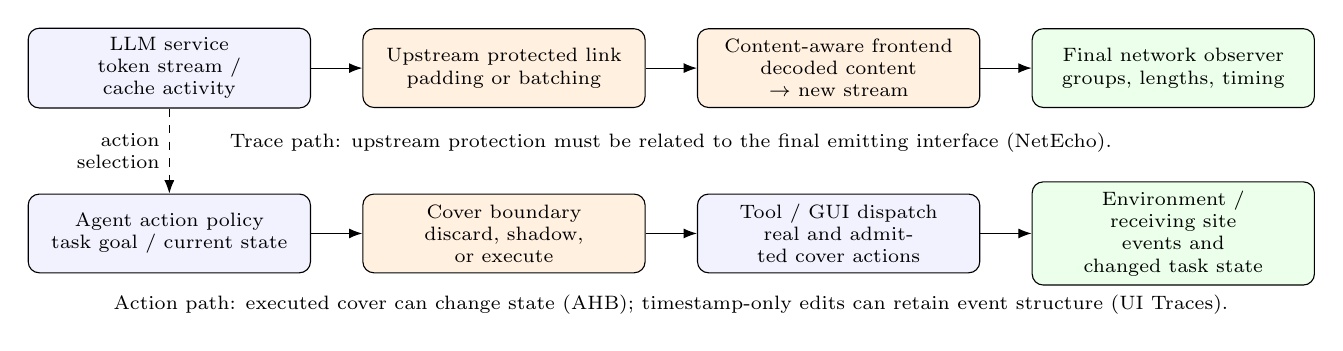
\begin{tikzpicture}[font=\scriptsize,>=Latex,
box/.style={draw,rounded corners,align=center,text width=3.35cm,minimum height=10mm,fill=blue!5},
boundary/.style={box,fill=orange!12},
observer/.style={box,fill=green!8}]
\node[box] (llm) at (0,0) {LLM service\\token stream / cache activity};
\node[boundary] (api) at (4.25,0) {Upstream protected link\\padding or batching};
\node[boundary] (front) at (8.5,0) {Content-aware frontend\\decoded content $\rightarrow$ new stream};
\node[observer] (net) at (12.75,0) {Final network observer\\groups, lengths, timing};
\draw[->] (llm)--(api);
\draw[->] (api)--(front);
\draw[->] (front)--(net);
\node[box] (policy) at (0,-2.1) {Agent action policy\\task goal / current state};
\node[boundary] (cover) at (4.25,-2.1) {Cover boundary\\discard, shadow, or execute};
\node[box] (dispatch) at (8.5,-2.1) {Tool / GUI dispatch\\real and admitted cover actions};
\node[observer] (state) at (12.75,-2.1) {Environment / receiving site\\events and changed task state};
\draw[->] (policy)--(cover);
\draw[->] (cover)--(dispatch);
\draw[->] (dispatch)--(state);
\draw[->,dashed] (llm.south)--node[left,align=right]{action\\selection}(policy.north);
\node[font=\scriptsize,align=center] at (6.37,-.95)
{Trace path: upstream protection must be related to the final emitting interface (NetEcho).};
\node[font=\scriptsize,align=center] at (6.37,-3.0)
{Action path: executed cover can change state (AHB); timestamp-only edits can retain event structure (UI Traces).};
\end{tikzpicture}

\caption{Observation and execution boundaries. The four demonstrations test emitter placement, stateful execution/link composition, real-agent operation signatures, and timing with matched transport controls.}
\label{fig:system-model}
\end{figure*}

\section{Scope and Systematization Method}\label{sec:methodology}\label{sec:background}
\subsection{Research questions, eligibility and threat polarity}
We organize the systematization around four questions: which hidden targets, threat polarities and auxiliary observables appear across LLM and agent systems (RQ1); how signal generation origin relates to receiver observation permissions (RQ2); which holdouts establish portability across tasks, configurations and hardware (RQ3); and when a component intervention protects an end-to-end workflow at a bounded utility and cost (RQ4).

Core inclusion requires five conjunctive criteria: (C1) LLM or agent execution, (C2) a hidden target property, (C3) an execution-dependent auxiliary observable rather than ordinary output semantics alone, (C4) specified observer permissions, and (C5) an empirical inference evaluation. Mixed-feature papers qualify only if they isolate an auxiliary-only C3 component; thus coding fingerprints, WildAuth, ZeroPrint, endpoint-content fingerprints and StepFinder remain adjacent boundary comparators \cite{ghaleb2026codingfingerprint,wang2026dialogue,shao2026zeroprint,leshin2026endpoint,zhu2026stepfinder}. Table~\ref{tab:boundary-rules} states the observable eligibility rules.
\begin{table}[t]\centering\footnotesize
\caption{Observable-based eligibility. A hidden target alone does not make a semantic attack a side channel.}\label{tab:boundary-rules}
\begin{tabularx}{\columnwidth}{@{}p{.39\columnwidth}Y@{}}\toprule
Observed input & Decision and required distinction\\\midrule
Length, timing, cache response & Core when measured execution dependence supports hidden-target inference.\\
Own-site actions & Core attribution with site permission; no automatic access to other sites or private tool logs.\\
Reply states the secret & Direct disclosure; adjacent, not auxiliary-channel evidence.\\
Reply style/content identifies a user & Adjacent unless a separately evaluated auxiliary mechanism is established. WildAuth stays a mixed-view comparator.\\
Output-filter membership oracle & Core only for an isolated accept/reject or differential-response oracle tied to filter execution; semantic content alone remains adjacent.\\
Privileged loop/fault logs & Separate diagnostic component when C1--C5 hold; does not increase confidentiality evidence.\\\bottomrule
\end{tabularx}\end{table}


We use four narrative groupings of objectives and observer roles, not mutually exclusive classes. An unauthorized identity inference can be both attribution and a confidentiality concern. Each record separately specifies the inference target, observer, authorization relation and protected interest:
\begin{enumerate}
\item \textbf{Type~I (Confidentiality and privacy protection):} An unauthorized observer attempts to infer private user prompts, personal traits, visited domains or proprietary model states; the defense protects user or tenant confidentiality (e.g., NetEcho, WRA, Early Bird, KVGov, CachePrune, OTRO \cite{netecho2025,jeong2026wra,earlybird2025,addagada2026kvgov,wu2026cacheprune,lee2026otro}).
\item \textbf{Type~II (Provenance and identity attribution):} An observer infers which model, agent harness or user identity generated a trace from timing, packet or DOM event structure (e.g., UI Traces, FP-Agent, AgentPrint, Lidar \cite{uitraces2026,wang2026fpagent,agentprint2025,wang2026lidar}).
\item \textbf{Type~III (Human--agent / bot-detection evasion):} The receiving platform operates a defensive classifier to detect automated bots, while the agent applies ``action humanization'' (e.g., AHB \cite{zhu2026turing}) to evade detection---inverting the defender/attacker polarity relative to Type~I privacy protection.
\item \textbf{Type~IV (Authorized operator diagnostics):} Privileged loop detection, serving root-cause localization or internal residual-stream monitoring (ClawGuard, cycle detection, LumiMAS, LLM RCA, MIRAGE \cite{gan2026clawguard,george2025cycles,solomon2026lumimas,scheinert2026rca,revankar2026mirage}), which use C1--C5 auxiliary signals for legitimate system telemetry rather than privacy exploitation.
\end{enumerate}

\subsection{Seed-anchored purposive corpus and exact reconciliation}
Because LLM and agent side-channel papers are scattered across security conferences, systems venues and preprints under heterogeneous terminology (``remote keylogging,'' ``prompt-cache leakage,'' ``workflow fingerprinting,'' ``agent humanization''), our corpus is constructed through \emph{purposive seed selection, venue-targeted proceedings screening (IEEE S\&P, USENIX Security, NDSS, ACM CCS, PMLR) and one-hop backward/forward citation snowballing} from 40 fixed seeds (2,237 backward reference occurrences and 24 distinct forward works screened; 38/40 forward seeds resolved; seed resolution and the number of distinct returned works are different counts), complemented by native database exports and bulk keyword searches (Appendix~\ref{app:search} and Supplement S1/S10).

To document why standalone Boolean keyword queries cannot replace seed-and-snowball discovery, we audited both our historical October 8--9 native IEEE/ACM exports and a completed October 21 supplementary search frame comprising four Semantic Scholar title/abstract bulk queries and two native arXiv searches (615 occurrences deduplicated to 565 unique records; Table~\ref{tab:corpus-reconciliation}). Those six supplementary keyword queries returned 17/24 of a fixed 24-paper core subset of our 40 seeds (\texttt{seed\_n=24}) and 25/60 of the October 8 snapshot. Because the 24 known papers are a core subset of the 40 initial seeds rather than an external holdout, 17/24 and 25/60 measure \emph{lexical overlap between narrow Boolean queries and our seed-anchored corpus}, not calibrated database recall: the two native arXiv queries required the exact hyphenated string \texttt{"side-channel"} (missing studies titled with ``prompt leakage,'' ``keylogging,'' ``timing attacks'' or ``fingerprinting''), and Semantic Scholar title/abstract matching did not search full texts of USENIX/NDSS PDFs.

\begin{table}[t]\centering\footnotesize
\caption{Item-by-item reconciliation of the 565-record October 21 search frame (before and after the 204-record exclusion audit) and the transition from the 60-family snapshot to all \FinalN{} coded families.}\label{tab:corpus-reconciliation}
\setlength{\tabcolsep}{3.5pt}
\begin{tabularx}{\columnwidth}{@{}Yrrr@{}}\toprule
Route / family category & Pre-audit & Audit $\Delta$ & Final (Indexed)\\\midrule
Excluded: no hidden C2/C3 target & 221 & $-4$ & 217 (0)\\
Excluded: outside LLM / diff.\ target & 175 & $0$ & 175 (0)\\
Existing snapshot core / adjacent & 23 / 1 & $+1 / 0$ & 24 / 1 (in 60)\\
New source-verified core families & 14 & $+1$ & 15 (\textbf{+15})\\
Adjacent source-reviewed contexts & 28 & $+2$ & 30 (\textbf{+7})\\
Adjacent metadata-only contexts & 28 & $0$ & 28 (0)\\
Background / proposal metadata & 58 & $0$ & 58 (0)\\
Missing abstract / unavailable text & 17 & $0$ & 17 (0)\\\midrule
\textbf{565-frame total / Net added families} & \textbf{565} & \textbf{0 net} & \textbf{565 (+22)}\\
\textbf{Coded collection}: Core / Adjacent (\textbf{Total}) & \multicolumn{3}{r}{Snapshot: 43 / 17 (\textbf{60}) $\to$ Full: \FinalCore{} / \FinalAdjacent{} (\textbf{\FinalN{}})}\\\bottomrule
\end{tabularx}
\par\smallskip\raggedright\footnotesize
The exclusion audit selected 177 high-risk pattern matches plus 27 reason-stratified records (seed 20261021), rather than all 396 initially excluded records. This enriched 204-record subset rerouted 4 records out of the 221 initial C2/C3 exclusions: (1) \texttt{SUP-0192} (MIRAGE \cite{revankar2026mirage}) moved to new core ($14+1=15$, all 15 added to the family index); (2) \texttt{SUP-0552} (InputSnatch arXiv alias) merged into existing family \texttt{inputsnatch2024} ($23+1=24$, $+0$ new families); and (3--4) \texttt{SUP-0191} and \texttt{SUP-0424} moved to source-reviewed adjacent contexts ($28+2=30$, of which 7 boundary-defining studies enter the adjacent index and 23 remain in the 565-record ledger). Thus $60 + 15\text{ (core)} + 7\text{ (adjacent)} = \FinalN{}$.
\end{table}

Table~\ref{tab:corpus-reconciliation} reconciles every record across the $60\to\FinalN{}$ transition. All \FinalCore{} core families (\FinalA{} workflow-origin, \FinalB{} inherited-runtime/application; 53 non-diagnostic and 5 Type~IV diagnostic) and \FinalAdjacent{} adjacent families are integrated into the unified corpus maps and intervention dispositions (Supplement S2/S5). Across the \FinalCore{} core families, 20 evaluate mitigations (16 snapshot families plus four additions). The result ledger is broader: 33 baseline records from 22 families, including six contextual comparators, plus six records from the four added mitigation families. Thus the 39-record ledger spans 26 families and 78 utility/cost field positions; the reporting-audit denominator is 20.

\subsection{Supplied coding records and agreement}
The supplied package records a primary AI-assisted coding workflow and a second coding column described by its provenance as a domain-expert review. We retain the recorded agreement summaries and supply their source columns. The files alone do not verify coder identity, blinding or independence from the primary decisions; we therefore report annotation agreement rather than newly verified independent human validation. The recorded scope is:
The saved screening sample has 93/100 three-class agreement ($\kappa=0.886$); the nine-item baseline audit has 134/144 cell agreement across 16 families ($\kappa=0.876$); and the 50-pair sample has 141/150 judgment agreement ($\kappa=0.916$). The latter covers all 13 same-family pairs plus 37 other within-cohort pairs. Full intervals and source locators remain in Supplement S8 and the annotation files.


The historical confidence intervals resample individual screening records, audit cells and pairwise judgments respectively. Cells within families and three judgments within a pair are dependent, so these intervals are conditional descriptive summaries, not cluster-robust generalization intervals. The 36 cells for four added families are outside the 144-cell agreement calculation. Agreement also does not establish coding correctness, and $\kappa$ depends on category prevalence.

\soktakeaway{SoK Takeaway 1 (Search and evidence scope)}{The supplementary queries returned 25/60 snapshot families and 17/24 known seed papers. These overlaps motivate complementary discovery methods; they neither estimate field-wide recall nor identify why each missing paper was absent. Objective, observer and authorization must be specified separately when comparing interventions.}

\section{Result Records, Comparability Rules and Validity}\label{sec:scope}
The atomic unit of our repository is one \emph{evaluated result record}, rather than a whole paper or a single headline score. A result record binds a source version and locator to seven structured fields: Source, Target (and threat polarity Types~I--IV), Receiver projection, Intervention boundary, Attacker training/calibration ($D_0$ vs.\ $D_2$), Workload/holdout, and Outcomes (inference metric, task/component utility, and cost object; Table~\ref{tab:result-record}). A study family contributes multiple records whenever it evaluates distinct execution modes (e.g., stored capture vs.\ live loopback in Dangol \cite{dangol2026workflow}), distinct mechanisms (e.g., $K$-prefix KV simulation vs.\ GPTCache semantic de-identification in Early Bird \cite{earlybird2025}), or separately scoped performance benchmarks (e.g., SafeKV \cite{chu2025safekv} and OTRO \cite{lee2026otro}).
\begin{table}[t]\centering\footnotesize
\caption{A single result record. Only fields relevant to the requested comparison must align; unavailable required fields remain unresolved.}\label{tab:result-record}
\begin{tabularx}{\columnwidth}{@{}p{.24\columnwidth}Y@{}}\toprule
Record field & Required meaning\\\midrule
Source & Family/result ID, version, source locator, reading scope and hash.\\
Target & Hidden property, inference goal and protection relation: confidentiality, attribution, human/agent distinction or authorized diagnosis.\\
Receiver & Actual permission and released representation, including session/document linkage and any auxiliary inputs.\\
Intervention & Where protection ends; whether edits affect stored traces, transmission or executed actions.\\
Attacker & Fit/calibration condition, test population, training access and adaptation budget.\\
Workload & Task, system, topology/hardware and grouping/holdout.\\
Outcomes & Inference metric / denominator; objective or proxy utility; applicable cost object; uncertainty and field states.\\\bottomrule
\end{tabularx}\end{table}


\paragraph{Indexing schema and comparison contracts}
The mnemonic \scope{} (Secret/target, Channel, Observer, Pipeline, Exploitation goal) names the target-and-channel columns of our index, paired with evaluation provenance. Generating layers span hardware (P1), serving (P2), transport (P3), application/API (P4), orchestration (P5), tools/MCP (P6), environment (P7) and multi-agent communication (P8). We apply three comparison contracts (Table~\ref{tab:comparison-contracts}): a comparison is \emph{compatible} when required fields align; \emph{incompatible} when a positive mechanism or boundary conflict is established (such as substituting token-payload ratios for wire bytes or offline timestamp edits for live action delays); and \emph{unresolved} when a required binding is unreported (\NRR{}), unavailable (\NRA{}) or unverified (\NRV{}). Table~\ref{tab:result-lineage} illustrates a complete record-to-judgment lineage.
\begin{table}[t]\centering\footnotesize
\caption{Comparison rules. A known mismatch and a missing binding have different consequences.}\label{tab:comparison-contracts}
\begin{tabularx}{\columnwidth}{@{}p{.28\columnwidth}Y@{}}\toprule
Requirement & Condition and resulting license\\\midrule
Descriptive comparison & Identify the shared target and receiving view. Describe differing populations or metrics separately; numerical cost comparisons additionally require aligned cost objects. Token payload and wire bytes cannot be ranked as the same cost.\\
Paired effect & Compare the same defended test units and outcome. A known test-unit mismatch makes that subtraction incompatible; an unverified fit binding leaves the effect unresolved.\\
Deployment transfer & Establish a bridge for the changed receiver, intervention, workload, topology or hardware. A demonstrated violation blocks the proposed transfer; an untested bridge leaves it unresolved. Permit only the range and endpoints actually covered.\\\bottomrule
\end{tabularx}\end{table}

\begin{table}[t]\centering\footnotesize
\caption{Filled record and its licensed judgment. Values are source-reported; no cross-mode effect is computed.}\label{tab:result-lineage}
\begin{tabularx}{\columnwidth}{@{}p{.24\columnwidth}Y@{}}\toprule
Join key / field & Entry\\\midrule
Family / result & Dangol workflow / \texttt{DANGOL-livebinding}.\\
Version / locator & arXiv:2606.07150v3, \S9.7, live-protocol paragraph after Table~5 \cite{dangol2026workflow}.\\
Target / view & Workflow classification from live Oblivious HTTP (OHTTP)/Agent-to-Agent (A2A) traffic; not GUI-state observation.\\
Intervention & Live fixed-rate cover with fresh per-session identifiers, distinct from transformed stored captures.\\
Workload / testbed & Workflow classes with client, relay, gateway and agent co-located on one loopback host.\\
Outcome / cost & Accuracy 0.30; about 13$\times$ bytes and 11$\times$ latency in that condition.\\
Unresolved fields & Objective terminal task utility \NRR{}; precise paired live-refit comparison \NRV{}.\\
Licensed judgment & These costs describe this live protocol condition. They neither price dummy GUI actions nor prove task preservation. A matched objective endpoint is needed for the latter.\\\bottomrule
\end{tabularx}\end{table}



\paragraph{Rule-application consistency check}
We exercise the comparison rules on 24 author-constructed cases spanning seven Compatible, twelve Incompatible and five Unresolved judgments. The two recorded coding columns match the case labels on 23/24 and 22/24 cases and agree on 21/24 ($\kappa=0.795$). This check documents how the rules resolve aligned results, explicit boundary conflicts and missing bindings; case-level outcomes and confusion matrices are in Supplement S7. The indexing exercise in S7 separately tests retrieval through the evidence schema.

\section{Corpus Map Across 82 Study Families}\label{sec:corpus-map}
\subsection{Origins, receiving projections and threat polarities}
Across all \FinalCore{} core families in our unified repository, 38 inherit runtime, serving or hardware channels (Origin~B), while 20 concern agent-workflow channels arising from orchestration, tool dispatch, browser navigation and multi-agent protocols (Origin~A; Table~\ref{tab:core-family-map}). Signal-generation origin is distinct from receiver location and threat polarity. The full map makes these distinctions visible family by family.
\begin{table*}[t]\centering\footnotesize
\caption{Complete map of the 58 core study families. Each family appears once; multiple layer/type labels describe different components or objectives within the family.}\label{tab:core-family-map}
\setlength{\tabcolsep}{3pt}
\begin{tabularx}{\textwidth}{@{}Ycc@{\hspace{1.5em}}Ycc@{}}\toprule
Core family & $G\,\to\,O$ & Type & Core family & $G\,\to\,O$ & Type\\\midrule
ArchSnoop~\cite{weng2026archsnoop} & $1\,\to\,1$ & \texttt{II} & PromptPeek~\cite{promptpeek2025} & $2\,\to\,4$ & \texttt{I}\\
Behind Bars~\cite{gu2026behindbars} & $1\,\to\,1$ & \texttt{I} & Remote keylogging~\cite{weiss2024prompt} & $2\,\to\,3$ & \texttt{I}\\
Edge EM leakage~\cite{alhalawani2026physicaledge} & $1\,\to\,1$ & \texttt{I} & Remote timing~\cite{carlini2024remote} & $2\,\to\,3$ & \texttt{I}\\
Energon~\cite{chaudhuri2025energon} & $1\,\to\,1$ & \texttt{II} & Routing metadata~\cite{chen2026routingmetadata} & $2\,\to\,4$ & \texttt{I}\\
I Know What You Said~\cite{gao2025iknow} & $1\,\to\,1$ & \texttt{I} & SafeKV~\cite{chu2025safekv} & $2\,\to\,4$ & \texttt{I}\\
MoEcho~\cite{ding2025moecho} & $1\,\to\,1$ & \texttt{I} & Speculative decoding~\cite{wei2024speculation} & $2\,\to\,3$ & \texttt{I}\\
PAGE404~\cite{nazaraliyev2026page404} & $1\,\to\,1$ & \texttt{I} & SpliceLeak~\cite{spliceleak2026} & $2\,\to\,4$ & \texttt{I}\\
Spill the Beans~\cite{spillbeans2025} & $1\,\to\,1$ & \texttt{I} & SplitDecoy~\cite{politis2026splitdecoy} & $2\,\to\,2$ & \texttt{I}\\
Detokenization Leaks~\cite{weiss2026detokenization} & $1,2\,\to\,1$ & \texttt{I} & Time Will Tell~\cite{timewilltell2024} & $2\,\to\,4$ & \texttt{I}\\
LLM-serving RCA~\cite{scheinert2026rca} & $1,2\,\to\,2$ & \texttt{IV} & Whisper Leak~\cite{whisperleak2025} & $2\,\to\,3$ & \texttt{I}\\
LLM-WFIN~\cite{jiao2025llmwfin} & $1,2\,\to\,1,3$ & \texttt{I} & MIRAGE~\cite{revankar2026mirage} & $2,5\,\to\,2$ & \texttt{IV}\\
OTRO~\cite{lee2026otro} & $1,2\,\to\,1$ & \texttt{I} & Cloud traffic benchmark~\cite{pouryousef2026traffic} & $2,5,8\,\to\,3$ & \texttt{I,II}\\
Shape and Substance~\cite{hadad2026shape} & $1,2\,\to\,1$ & \texttt{I} & Web-agent unmasking~\cite{fayolle2026webagents} & $3,7\,\to\,3,7$ & \texttt{II,III}\\
SparLeak~\cite{chen2026sparleak} & $1,2\,\to\,1$ & \texttt{I} & LumiMAS~\cite{solomon2026lumimas} & $4,5\,\to\,4,6$ & \texttt{IV}\\
SparSEEty~\cite{jo2026sparseety} & $1,2\,\to\,1$ & \texttt{I} & AgentPrint~\cite{agentprint2025} & $5\,\to\,3$ & \texttt{I,II}\\
TDXRay~\cite{hornetz2026tdxray} & $1,2\,\to\,1$ & \texttt{I} & Cycle detection~\cite{george2025cycles} & $5\,\to\,4,6$ & \texttt{IV}\\
ClawGuard~\cite{gan2026clawguard} & $1,5\,\to\,1$ & \texttt{IV} & AgentProv~\cite{wang2026agentprov} & $5,6\,\to\,6$ & \texttt{II}\\
Cache contention~\cite{abubakar2026contention} & $2\,\to\,4$ & \texttt{I} & Lidar~\cite{wang2026lidar} & $5,6\,\to\,6$ & \texttt{II}\\
CachePrune~\cite{wu2026cacheprune} & $2\,\to\,4$ & \texttt{I} & ProcGrep~\cite{oderinwale2026procgrep} & $5,6\,\to\,4,6$ & \texttt{II}\\
Early Bird~\cite{earlybird2025} & $2\,\to\,4$ & \texttt{I} & SIGLEAK~\cite{geng2026sigleak} & $5,6\,\to\,4,6$ & \texttt{I}\\
InputSnatch~\cite{inputsnatch2024} & $2\,\to\,4$ & \texttt{I} & Campaign attribution~\cite{park2026crosscampaign} & $5,6,8\,\to\,6,8$ & \texttt{II}\\
KVGov~\cite{addagada2026kvgov} & $2\,\to\,2,4$ & \texttt{I} & Dangol workflow~\cite{dangol2026workflow} & $5,6,8\,\to\,3,6,8$ & \texttt{I}\\
Leaky Language Models~\cite{majidi2026leakylms} & $2\,\to\,4$ & \texttt{I} & AgentTell~\cite{shahriar2026agenttell} & $5,7\,\to\,7$ & \texttt{I}\\
LLMs Have Rhythm~\cite{alhazbi2025rhythm} & $2\,\to\,3$ & \texttt{II} & AHB~\cite{zhu2026turing} & $5,7\,\to\,7$ & \texttt{III}\\
ML privacy channels~\cite{debenedetti2024privacy} & $2\,\to\,4$ & \texttt{I} & FP-Agent~\cite{wang2026fpagent} & $5,7\,\to\,7$ & \texttt{II}\\
MoE prompt stealing~\cite{yona2024stealing} & $2\,\to\,4$ & \texttt{I} & PersonaFingerprint~\cite{song2026personafingerprint} & $5,7\,\to\,3$ & \texttt{I}\\
NetEcho~\cite{netecho2025} & $2\,\to\,3$ & \texttt{I} & UI Traces~\cite{uitraces2026} & $5,7\,\to\,7$ & \texttt{II}\\
Prompt Echo~\cite{prompt_echo2026} & $2\,\to\,3$ & \texttt{I} & Whose Agent?~\cite{kang2026whoseagent} & $5,7\,\to\,7$ & \texttt{II}\\
Prompt-cache audit~\cite{gu2025promptcaching} & $2\,\to\,4$ & \texttt{I} & WRA~\cite{jeong2026wra} & $5,7\,\to\,3$ & \texttt{I}\\
\bottomrule\end{tabularx}
\par\smallskip\raggedright $G$ denotes signal-generation layers and $O$ the receiving observation layers. Layer indices: 1 hardware; 2 serving/runtime; 3 transport; 4 application/API; 5 orchestration; 6 tools; 7 browser/environment; 8 multi-agent communication. Types: I confidentiality/privacy; II attribution; III human--agent distinction/evasion; IV authorized diagnostics. These are objectives and observer roles, not mutually exclusive security guarantees. Privileged operator receivers and physical receivers are marked by the layer they inspect. Source versions, locators and the normalization of prose-only layer descriptions are in the artifact.
\end{table*}


\paragraph{Cross-origin synthesis}
Origin B includes token/packet lengths, cache timing and co-resident hardware channels; Origin A includes visited domains, tool dispatch and browser actions. Receiver permissions cut across these origins: a remote network observer, a same-site script and a privileged diagnostic hook expose different views even when they share an attribution target. Thus Origin A/B cannot substitute for Types I--IV or observer permissions. WRA's read-only privacy decoys, AHB's stateful evasion and SplitDecoy's exposed return path illustrate transfers that fail when these axes are collapsed \cite{jeong2026wra,zhu2026turing,politis2026splitdecoy}. The map retains every core family rather than using these examples as a substitute for coverage.

Layer incidence highlights where the systematization's comparison problem arises. In the 58-family map, signal-generation labels cluster at P2 serving/runtime (32 families) and P5 orchestration (19); receiving views cluster at P4 application/API (18), P1 hardware (16), and P3 transport (14). Generation at P3/P4 is rare (one family each), despite frequent observation at those layers. This source/receiver asymmetry makes the transfer question concrete: protection at a frequent source layer cannot be presumed to cover a different receiving projection. The map records layer sets, so it does not assign a causal edge to each source/receiver pair.

Purpose labels further show why a single “agent side channel” category is insufficient: Type I appears 41 times, Type II 13, Type III 2, and Type IV 5. The 32 map-only families extend coverage beyond mitigation comparisons: 15 list serving origins, 11 hardware and 11 orchestration; 19 concern confidentiality, nine attribution, one evasion and all five authorized-diagnostic families. They comprise 22 families without a scoped mitigation evaluation, five diagnostics, four unbound quantitative assertions, and SplitDecoy's boundary case (\S\ref{sec:defenses}). Mapping these families locates privacy targets, operator capabilities and candidate validation environments even when no scoped mitigation record enters the ledger. Counts are overlapping family-label incidences; the audit then applies its reuse rules to the 39 scoped result records.

\subsection{Relationship to prior systematizations}
Prior surveys establish compound-system threat models and confidential-computing boundaries. Banerjee et al.\ categorize cross-layer compound AI threats under MITRE tactics; Forough et al.\ distinguish TEE isolation boundaries from side-channel resistance and note that inference protections need not cover agent memory or action coordination \cite{banerjee2024compound,forough2026secrets}. Kotevska et al.\ propose a six-element privacy contract (asset, observer, channel, permitted disclosure, guarantee, evidence), with composition conditions framed as formal conjectures \cite{kotevska2026privacyfoundations}. Classical website-fingerprinting studies establish bandwidth/latency costs for transport shaping, including Tamaraw, WTF-PAD, FRONT and Walkie-Talkie \cite{cai2014systematic,juarez2016wtfpad,gong2020front,wang2017walkietalkie}. Our contribution is to make reuse decisions inspectable across 82 mapped families and 39 source-bound result records, then organize the empirical checks around four boundaries: emitter and transport; stateful execution and the exposed link; repeated real-agent trajectories; and live timing with adapted website-fingerprinting controls. This evidence map shows why a defense's name or layer is insufficient for transfer: the receiver projection, state effects, workload and cost object must also align. Our experiments test these specific comparison obligations on a loopback TLS path and a pinned stateful tool simulator. These measurements connect established mechanisms to the cost and residual inference observed in streamed LLM and agent traffic.

\section{Three Deployment Case Studies}\label{sec:discussion}
Applying our repository schema to the literature resolves apparent contradictions across three fundamental deployment decisions (Table~\ref{tab:synthesis-decisions}): (1) when upstream traffic shaping survives downstream workflow hops; (2) why read-only query decoys and live GUI humanization produce opposite task outcomes; and (3) how adaptive retraining ($D_2$) and mechanism-specific cost boundaries govern operating-point selection.

\subsection{Case 1: bind the final target-bearing emitter}
\paragraph{The downstream re-emission boundary}
When an upstream LLM API applies record padding or token batching, does that protection cover the user-facing connection after an application frontend? NetEcho demonstrates that a content-aware frontend that consumes decoded upstream tokens and re-serializes responses into new chunks (Trace~A token counts per group; Trace~B character lengths) restores topic and conversation distinguishability \cite{netecho2025}. SplitDecoy establishes the same boundary on a backward return path: even when forward split-model activations are obfuscated with decoys, the returned backward gradient exposes nonzero row support on every tested frame across nine seeds \cite[Sections 5.1--5.3]{politis2026splitdecoy}.

\noindent\textbf{Proposition 1 (target-oblivious postprocessing bound).}
Let $S$ be the hidden target, $Z$ the complete protected upstream representation and $Y$ the downstream observation. If $S\to Z\to Y$ forms a Markov chain (any downstream framing or randomization is conditionally independent of $S$ given $Z$), then by the data processing inequality \cite[Theorem~2.8.1]{cover2006elements},
\[
 I(S;Y)\leq I(S;Z).
\]
A content-aware frontend that decrypts, strips padding and re-chunks plaintext ($S\to (Z,\text{plaintext})\to Y$), or a backward pass that computes gradients from unprotected loss masks, need not satisfy $I(S;Y\mid Z)=0$. The sufficient-condition theorem then ceases to certify the bound; leakage must be checked separately. Section~\ref{sec:controlled-placement} demonstrates the specified re-emission mechanism on TLS~1.2 sockets.

\subsection{Case 2: resolve the WRA versus AHB cover asymmetry}
\paragraph{Two axes of asymmetry: threat polarity and action risk}
A comparison that groups WRA's decoy requests \cite{jeong2026wra} and AHB's humanized actions \cite{zhu2026turing} together as ``cover traffic'' can create an apparent paradox: WRA reports a clean privacy improvement (one concurrent decoy reduces functional-intent reconstruction $E_{\rm func}$ from 0.770 to 0.610), whereas AHB reports severe task collapse (Trip Planning success falls from 0.75 Raw to 0.15 under combined \texttt{Online+Fake} humanization).

Binding their result records shows that WRA and AHB sit at opposite poles along \emph{two structural axes}:
\begin{enumerate}
\item \textbf{Threat polarity inversion (Type~I vs.\ Type~III):} WRA is a Type~I privacy defense protecting a user's research intent from a network/domain observer. AHB is a Type~III bot-evasion mechanism designed to make an automated mobile GUI agent mimic human touch patterns so it bypasses platform anti-automation controls.
\item \textbf{Action-interface risk magnitude (discarded read-only queries vs.\ live GUI state mutations):} WRA's decoys are \emph{read-only search and retrieval prompts} whose returned pages are discarded locally before synthesis; they never invoke state-mutating tools on the user's account. By contrast, AHB's \texttt{Fake} operator injects \emph{unfiltered live GUI touch events} directly onto stateful mobile application screens, triggering unintended navigation and form submissions. The non-Fake \texttt{History+Long} configuration changes timing/trajectory history. These source-reported condition rates are not treated as a matched effect: condition-specific sample denominators were not independently recovered in this revision.
\end{enumerate}

\paragraph{Dispatch-time authorization versus terminal-state scoring}
Separating cover execution routes also exposes a fundamental \emph{analytical design argument} regarding agent benchmark evaluators: terminal state-snapshot scorers (such as $\tau$-bench's native reward, which hashes the final database state against the reference state) are \textbf{path-oblivious}. If an unconfirmed live cover action happens to perform the exact state transition that the user's task later intended (or preempts a real action so the real action fails with a status error while leaving the terminal state identical to baseline), a terminal-snapshot scorer awards a perfect score of $1.0$ although the endpoint does not establish authorization of the earlier call. Systems admitting cover to live dispatch must therefore enforce authorization and provenance checks at dispatch time and inspect tool state-machine transitions (such as one-way status flags or append-only audit ledgers, demonstrated in Section~\ref{sec:tau-cover-bridge}).

\subsection{Case 3: bind adaptive retraining ($D_2$) and cost objects}
\paragraph{The $D_0\to D_2$ rebound and component-cost boundaries}
Selecting a defense operating point requires pairing an adaptive attacker evaluation (comparing a clean-trained classifier $D_0$ against a defended-trained classifier $D_2$ on the \emph{exact same defended test set}) with the cost of the actual deployed mechanism. In UI Traces \cite{uitraces2026}, retraining on timestamp-delayed archive traces ($D_2$) recovers substantial model-attribution accuracy (confirmed by our supplementary archive reanalysis on 1,135 test records: $+0.1503$ nats log-loss reduction over $D_0$, 98.333\% Bonferroni-adjusted CI (three contrasts) $[0.1205,0.1815]$; Supplement S4). Section~\ref{sec:controlled-placement} gives a matched TLS adaptation example. The separate retail study shows why prior-based baselines and rule attacks must accompany a learned observer; an improvement over $D_0$ alone does not establish useful inference.

On the cost side, record binding prevents cross-mechanism price substitution: Early Bird's $6$ms/$4\%$ GPTCache semantic de-identification overhead does not price $K$-prefix KV-cache isolation \cite{earlybird2025}; KVGov's $1.3\,\mu$s HMAC key-derivation microcost omits workload-dependent lost cache reuse \cite{addagada2026kvgov}; and SpliceDefense's $<5$ms/$<1\%$ QCP padding overhead prices chunk padding rather than combined CTBF+QCP deployment \cite{spliceleak2026}. Conversely, CachePrune jointly binds marked-token attack suppression, QA/summarization utility and serving throughput on selective KV sharing \cite{wu2026cacheprune}, and OTRO bounds conditional access-count leakage ($3.94\to 0.04$ bits given byte length) alongside separately scoped unpadded TTFT ($4.59\%$) and epoch-padding ($2.8$ms) costs \cite{lee2026otro}.
\begin{table*}[t]\centering\footnotesize
\caption{Source-local findings, cross-study synthesis and the resulting measurement obligation. These are reuse judgments, not accusations that the source authors claimed end-to-end protection.}\label{tab:synthesis-decisions}
\begin{tabularx}{\textwidth}{@{}p{.14\textwidth}YYY@{}}\toprule
Check & Source-local evidence and locator & Synthesis added by record separation & Changed judgment / controlled evidence\\\midrule
1. Receiver & NetEcho IV-C--E/Fig.5: frontend re-emission; SplitDecoy 5.1--5.3: backward gradient support. & Protected upstream and forward views do not cover newly exposed downstream or backward inputs. & Bind the final observer or prove the postprocessing condition. Two-link TLS placement reproduces this mechanism; costs use identical texts.\\
2. Execution & WRA 8.1/Table8: read-only query decoys; AHB 5.2.3/Table1/E.3: live GUI humanization. & Objectives, live action semantics and protected state scopes differ, so their utility outcomes are not contradictory. & Evaluate task objects, full account and shared database separately. Retail same-item writes change status; known-position filtering defeats cover in the specified dispatch view.\\
3. Adaptation and cost & UI Traces 6.1: delayed-trace refit; Dangol 9.7: capture versus live protocol; Early Bird's KV-prefix versus semantic-cache mechanisms. & A paired attack contrast requires the same defended tests; costs from another mode or mechanism cannot price the claimed protection. & Keep source-local comparisons and mark missing bridges unresolved. TLS adapted accuracy remains 70.8\% under 1024B buckets; the retail class-prior baseline exceeds the legacy learned accuracy.\\\bottomrule
\end{tabularx}\end{table*}


\section{Comparability Audit Across All 58 Core Families}\label{sec:defenses}
\subsection{Unified 58-core disposition and 39-record ledger}
The corpus partitions as $82=58$ core $+24$ adjacent families. Within the core, $58=20$ mitigation $+6$ contextual-record $+32$ map-only families; the result ledger contains $39=33+6$ records, respectively, from the first two groups. The six are SIGLEAK, AgentTell, FP-Agent, Behind Bars, LLMs Have Rhythm and ML privacy channels \cite{geng2026sigleak,shahriar2026agenttell,wang2026fpagent,gu2026behindbars,alhazbi2025rhythm,debenedetti2024privacy}. They supply fixed-guardrail, access-control, interference, VPN or filter-origin contrasts rather than the audited mitigation claim. The remaining 32 comprise 22 without a scoped mitigation evaluation, five diagnostics, four unbound assertions and SplitDecoy's boundary case. S18 maps every family and record. Table~\ref{tab:defense-types} groups mechanisms; Table~\ref{tab:family-audit} reports the 20-family audit.
\begin{table*}[t]\centering\footnotesize
\caption{Seven privacy and attribution intervention categories organized by receiving view and supported deployment judgment. Type I protects confidentiality; Type II addresses provenance or identity attribution.}\label{tab:defense-types}
\begin{tabularx}{\textwidth}{@{}p{.17\textwidth}p{.29\textwidth}Y@{}}\toprule
Intervention \& polarity & Evaluated view, target and source & Established result and applicable boundary\\\midrule
Padding / batching (Type~I: confidentiality) & Network packet lengths and groups; topic inference. NetEcho and Whisper Leak \cite{netecho2025,whisperleak2025}. & Collected padding traces retain inference signal; packet-group batching is evaluated by replay. A protected upstream length view does not cover downstream re-emission or residual grouping. Live incremental cost remains \NRR{}.\\
Constant-rate / transport cover (Type~I: confidentiality) & Network workflow fingerprint; Dangol's OHTTP testbed \cite{dangol2026workflow}. & The co-located loopback setting yields 0.30 recovery at about $13\times$ bytes and $11\times$ latency. Transformed-capture results are separate; neither result supplies objective agent-task utility.\\
Concurrent query decoys (Type~I: confidentiality) & Destination/domain observer; private prompt and trait inference. WRA \cite{jeong2026wra}. & Real/decoy research prompts execute in parallel as read-only queries whose decoy answers are discarded locally; interleaved-domain evaluation reduces one-decoy $E_{\rm func}$ from 0.770 to 0.610. Real output is retained; task completion under decoy load and execution cost remain unbound.\\
Cache isolation / keying (Type~I: confidentiality) & Co-tenant prefix timing; SafeKV, KVGov and CachePrune \cite{chu2025safekv,addagada2026kvgov,wu2026cacheprune}. & SafeKV reports post-trigger AUC near 0.5 and separate TTFT/throughput comparisons. KVGov's HMAC median $1.3\,\mu$s prices key computation, excluding lost reuse. CachePrune jointly binds marked-token protection, QA/summarization utility and serving performance.\\
Cache timing equalization (Type~I: confidentiality) & Co-tenant cache-fusion timing; SpliceDefense \cite{spliceleak2026}. & Constant-Time Boundary Fusion (CTBF) suppresses the tested signal over 15 tasks/75 steps. Quantized Chunk Padding (QCP) adds mean 7.5 tokens and $<5$ms/$<1\%$ prefill time; this does not price combined deployment.\\
Timestamp perturbation (Type~II: attribution) & Recorded website action metadata; model/agent attribution. UI Traces \cite{uitraces2026}. & Fitting on delayed traces ($D_2$) recovers substantial attribution performance under offline timestamp edits that retain action types/order. Live execution delay and task outcomes are not measured by the trace transformation.\\
Oblivious / unshared memory (Type~I: confidentiality) & Host or local resource observations; TDXRay, Gao et al.\ and OTRO \cite{hornetz2026tdxray,gao2025iknow,lee2026otro}. & TDXRay measures oblivious-map lookup cost; Gao measures loading/memory cost after disabling zero-copy. OTRO reduces conditional access-count information (3.94 to 0.04 bits) with separate unpadded TTFT (4.59\%) and epoch-padding ($2.8$ms) bounds.\\\bottomrule
\end{tabularx}
\par\smallskip\raggedright\footnotesize
Authorized operator diagnostics (Type~IV: ClawGuard, cycle detection, LumiMAS, LLM-serving RCA and MIRAGE) are baseline telemetry rather than privacy attacks or evasion defenses, and are cataloged separately.
\end{table*}


\subsection{Within-family and within-cohort record comparisons}
While the machine-readable audit retains all $\binom{33}{2}=528$ baseline pairs for completeness, 426 pairs cross unrelated mechanism cohorts and are outside scope by construction. The 13 within-family pairs are included in the 102 within-cohort pairs: $528=426+102$, with no additional subtraction of 13. Focusing on the \textbf{13 within-family pairs} (multiple records inside the same paper) and \textbf{102 within-cohort related pairs} (66 traffic-envelope, 28 cache-service, 3 behavioral-humanization, 3 generator-fingerprint, 1 local-memory, 1 fixed-instruction; Supplement S8) reveals why paper-level comparisons fail:
\begin{itemize}
\item Even within the \textbf{13 same-family pairs} ( plus 2 same-family pairs in the additions: \texttt{CACHEPRUNE-selective} vs.\ \texttt{CACHEPRUNE-context} and \texttt{OTRO-unpadded} vs.\ \texttt{OTRO-epochpad}), nearly half (6/13 baseline; 7/15 full) measure different primitives, targets or cost objects (e.g., Early Bird's $K$-prefix oracle simulation vs.\ its GPTCache semantic prototype; SpliceDefense's CTBF signal suppression vs.\ QCP-only prefill cost; OTRO's unpadded TTFT vs.\ derived epoch-padding cost).
\item Among the seven aligned-outcome same-family pairs, four evaluate different collection or execution populations (e.g., Dangol's stored-capture feature ablation at 0.17 accuracy vs.\ live loopback OHTTP at 0.30 accuracy) and three lack a verified matched-test binding, so none licenses cross-record subtraction as a single paired deployment effect.
\item Across the \textbf{102 related-cohort pairs}, only 16 (15.7\%) support a source-qualified descriptive comparison, whereas 80 (78.4\%) exhibit positively established receiver, target or cost-object mismatches and 6 (5.9\%) remain unresolved (the supplied 50-pair subsample, not all 102 pairs, has 94.0\% agreement across its 150 judgments, $\kappa=0.916$).
\end{itemize}

\subsection{Nine-item split reporting audit across 20 mitigation families}
Table~\ref{tab:family-audit} reports all 180 family/item bindings. R1--R9 specify the evidence needed for scoped reuse claims, separately from deployment Checks~1--3. R4 records protected-condition fitting; R5 records a matched clean-versus-adapted contrast on defended tests. R7--R9 record inference, utility and cost. A family-level Bound entry means at least one scoped result meets the item, not that every result in that family does.
\begin{table}[t]\centering\footnotesize
\caption{Per-family evidence bindings for all 20 evaluated-mitigation families. R1--R9 are scoped reuse items, not overall paper scores.}\label{tab:family-audit}
\setlength{\tabcolsep}{2.2pt}
\begin{tabularx}{\columnwidth}{@{}Y*{9}{c}@{}}\toprule
Family & R1 & R2 & R3 & R4 & R5 & R6 & R7 & R8 & R9\\\midrule
UI Traces~\cite{uitraces2026} & $\bullet$ & \auditpartial & $\bullet$ & $\bullet$ & $\bullet$ & $\bullet$ & $\bullet$ & $\circ$ & --\\
WRA~\cite{jeong2026wra} & $\bullet$ & \auditpartial & $\bullet$ & -- & -- & \auditpartial & $\bullet$ & \auditpartial & $\circ$\\
NetEcho~\cite{netecho2025} & $\bullet$ & $\bullet$ & $\bullet$ & $\bullet$ & \auditpartial & $\bullet$ & $\bullet$ & $\circ$ & $\circ$\\
Early Bird~\cite{earlybird2025} & $\bullet$ & $\bullet$ & $\bullet$ & $\bullet$ & \auditpartial & $\bullet$ & $\bullet$ & $\circ$ & $\bullet$\\
Whisper Leak~\cite{whisperleak2025} & $\bullet$ & $\bullet$ & \auditpartial & ? & ? & $\bullet$ & $\bullet$ & $\circ$ & $\bullet$\\
SpliceLeak~\cite{spliceleak2026} & $\bullet$ & $\bullet$ & $\bullet$ & -- & -- & $\bullet$ & $\bullet$ & $\circ$ & $\bullet$\\
Time Will Tell~\cite{timewilltell2024} & $\bullet$ & $\bullet$ & $\bullet$ & ? & ? & $\bullet$ & $\bullet$ & $\circ$ & $\bullet$\\
I Know What You Said~\cite{gao2025iknow} & $\bullet$ & $\bullet$ & $\bullet$ & -- & -- & $\bullet$ & $\circ$ & -- & $\bullet$\\
Speculative decoding~\cite{wei2024speculation} & $\bullet$ & $\bullet$ & \auditpartial & ? & ? & $\bullet$ & $\bullet$ & -- & $\bullet$\\
Dangol workflow~\cite{dangol2026workflow} & $\bullet$ & $\bullet$ & $\bullet$ & $\bullet$ & $\bullet$ & $\bullet$ & $\bullet$ & $\circ$ & $\bullet$\\
Cloud traffic benchmark~\cite{pouryousef2026traffic} & $\bullet$ & \auditpartial & ? & ? & ? & \auditpartial & $\bullet$ & \auditpartial & $\circ$\\
Remote timing~\cite{carlini2024remote} & $\bullet$ & $\bullet$ & $\bullet$ & -- & -- & $\bullet$ & $\bullet$ & $\circ$ & \auditpartial\\
TDXRay~\cite{hornetz2026tdxray} & $\bullet$ & $\bullet$ & $\bullet$ & -- & -- & $\bullet$ & $\circ$ & $\bullet$ & $\bullet$\\
SafeKV~\cite{chu2025safekv} & $\bullet$ & $\bullet$ & $\bullet$ & -- & -- & $\bullet$ & $\bullet$ & $\circ$ & $\bullet$\\
AHB~\cite{zhu2026turing} & $\bullet$ & $\bullet$ & $\bullet$ & \auditpartial & ? & $\bullet$ & $\bullet$ & $\bullet$ & $\circ$\\
KVGov~\cite{addagada2026kvgov} & $\bullet$ & $\bullet$ & $\bullet$ & -- & -- & $\bullet$ & $\bullet$ & $\circ$ & $\bullet$\\
CachePrune~\cite{wu2026cacheprune} & $\bullet$ & $\bullet$ & $\bullet$ & -- & -- & $\bullet$ & $\bullet$ & $\bullet$ & $\bullet$\\
OTRO~\cite{lee2026otro} & $\bullet$ & $\bullet$ & $\bullet$ & -- & -- & $\bullet$ & $\bullet$ & -- & \auditpartial\\
SparLeak~\cite{chen2026sparleak} & $\bullet$ & $\bullet$ & $\bullet$ & ? & ? & $\bullet$ & $\bullet$ & \auditpartial & $\circ$\\
Shape and Substance~\cite{hadad2026shape} & $\bullet$ & $\bullet$ & \auditpartial & ? & ? & $\bullet$ & \auditpartial & $\circ$ & \auditpartial\\
\midrule Bound & 20 & 17 & 16 & 4 & 2 & 18 & 17 & 3 & 11\\
Applicable & 20 & 20 & 20 & 11 & 11 & 20 & 20 & 17 & 19\\
\bottomrule\end{tabularx}
\par\smallskip\raggedright $\bullet$: bound; \auditpartial: partial; $\circ$: unreported in inspected scope; ?: unverified binding; --: inapplicable. R1 target/polarity; R2 receiver; R3 placement/execution; R4 defended-condition fit; R5 matched adaptation; R6 workload/generator shifts; R7 inference; R8 utility; R9 cost. A bound cell is supported by at least one scoped record. Dangol R5 concerns stored capture; its live-refit binding remains unverified. CachePrune jointly binds R7--R9 at one operating point.
\end{table}


For Dangol, R5 is Bound for in-fold stored-capture experiments; the live-refit paired comparison in Table~\ref{tab:result-lineage} remains \NRV{}. These are different records, so we retain the family count of two and explicitly restrict its meaning.

\soktakeaway{SoK Takeaway 2 (Joint evaluation gap)}{Across 20 mitigation families, 17 bind inference outcomes, 11 bind cost, 3 bind utility and 2 bind a matched adaptation contrast. Excluding structurally inapplicable entries, the latter three rates are 11/19, 3/17 and 2/11. \NRV{} means unverified binding, not an absent experiment. CachePrune binds inference, utility and cost at one operating point; this is not a claim that it also binds adaptive evaluation.}

\section{Systematic Holdout Evidence for Transfer}\label{sec:evaluation}\label{sec:threats}
\subsection{Six axes across all 82 families}
Appendix~\ref{app:holdouts} gives the complete family-by-axis matrix, including the 24 adjacent families. It codes task/input/user, model, harness/topology, hardware, network/load and time separately from the archived source-bound extraction. H denotes an explicitly reported held-out unit/domain; V a condition comparison or recalibration; X a scoped restriction; ? unresolved extraction. H does not certify every grouping detail or successful transfer, and ? is never counted as absence. Conceptual families receive an inapplicable dash.

The matrix contains H entries for 13 families on task/input/user, three on model, two on harness/topology and one on network; none is resolved as H for hardware or time. The latter axes contain seven V entries each: calibration, condition sweeps and temporal observations already exist in the literature. With 73 hardware and 71 temporal entries unresolved, this is a map of \emph{documented evidence}, not a claim that those papers omitted such tests. Multiple H entries are counted once per family/axis, not pooled as independent experiments.

\subsection{What each holdout licenses}
Whisper Leak holds out target prompts; FP-Agent has a separate task holdout but unresolved visitor/host separation. Dangol's leave-composition-out and the traffic benchmark's topology shift change a different generator \cite{whisperleak2025,wang2026fpagent,dangol2026workflow,pouryousef2026traffic}. LLM-Fin and ArchSnoop test unseen variants/configurations within known model families; LeakyLMs conditions architecture inference on known GPU type and calibration \cite{nazari2024llmfin,weng2026archsnoop,majidi2026leakylms}. Thus a positive model holdout does not establish unknown-hardware transfer. UI Traces' recorded question overlap further shows why task labels and actual held-out units must remain distinct \cite{uitraces2026}.

\subsection{Operational consequence}
Select the axis changed by deployment, require a source-bound separation on that axis, then check whether fitting or calibration crossed the split. Otherwise scope the result to its observed condition. Feature ablations and additional models alone supply V evidence, not a bridge to an unseen generator. This rule also governs our endpoint experiments: within-model refits, source-trained attacker transfer and source-calibration transfer occupy separate matrix cells. The systematic result is the mismatch between the requested transfer axis and the available evidence, not a ranking by the number of holdouts.

\paragraph{From holdout counts to a transfer obligation}
Each axis names a distinct source of variation. A task holdout tests new inputs under its stated generator; a model holdout changes the generator; topology and network holdouts change the receiving path; hardware and time can change the implementation or scheduling process. The 13 task/input H entries and three model H entries therefore answer different questions, rather than form a single robustness score. Where extraction remains unresolved, the next action is to establish the source's scope before demanding a new experiment. Where a deployment changes several axes, evidence must cover their intended combination: separate model and network tests do not automatically establish their joint operating point.

\section{Controlled Transfer Tests}\label{sec:controlled-placement}\label{sec:tau-cover-bridge}
The experiments operationalize the audit's three bindings: observation, execution and matched evaluation. E5--E7 isolate mechanisms using saved outputs and reference programs; E9 evaluates real LLM-generated trajectories with training-only calibration. Seven author-written judgments were recorded before E5--E7; their reassessment is retained in Supplement S12. These cases test mechanisms, not the audit's external decision accuracy.

For E6/E7/E9, a cell meets the \emph{evaluated-suite criterion} when maximum BA has an upper 95\% bound below 0.60 and maximum AUROC is below 0.65. A lower BA bound above 0.60 indicates above-threshold leakage; other cells are inconclusive. We recompute the suite maximum within each of 2,000 common bootstrap draws: tasks for E6/E7 and customers for E9, retaining their tasks and repeats together. Intervals condition on fitted predictions and do not cover unknown attackers.

A byte-transparent relay captures post-handshake TLS application records on loopback connections. TLS~1.3 session tickets are disabled. E5--E8 use saved text or stand-in planners; E9 invokes a real model and executes its structured actions in the local public retail simulator. No production account or tool is modified.

\subsection{Transport: buffered and streaming emitters}
\paragraph{Buffered emitter}
The corpus has one prompted brief and one prompted expanded \texttt{gpt-6-luna} response for each of 24 topics (12 training and 12 test topics); these are designed conditions, not natural length samples. In a two-link TLS~1.2 replay, a frontend that decodes and re-chunks the upstream text leaves the terminal link 100\% separable when only the upstream link is padded; padding both links reduces the evaluated classifier to 50\%. This reproduces NetEcho's mechanism \cite{netecho2025}. With workload-matched denominators, 512-byte buckets cost 2.30$\times$ and 1.43$\times$ for two sentence-prefix workloads (T2, T3); a cap fitted on training lengths (1,280 bytes) yields 50\% at 2.18$\times$ for verbosity (T1). Under offsets, 1024-byte buckets and random tails, refitting ($D_2$) gains 13.5--50.0 points over $D_0$; constant caps give no gain. Supplement S11 retains all cells.

\paragraph{E5: the same texts as a token stream}
These figures describe an emitter that frames a response only after generation is complete. LLM APIs usually stream, and the streaming attacks in our corpus observe per-token records \cite{weiss2024prompt,whisperleak2025}. E5 emits the same 48 texts as server-sent chunk events, one TLS record per token, over TLS~1.2 (AES-128-GCM) and TLS~1.3 (AES-256-GCM). Token boundaries use o200k\_base as a proxy; the generating model's tokenizer and timing were not saved, so latency is reported in token intervals. The framings are per-event random padding of 1--64 bytes (an obfuscation field), a constant 144-byte event, 8-token batches padded to a constant size, and constant events plus dummy events up to the largest training token count. Besides $D_0$ and $D_2$ threshold and sequence classifiers, a closed-world attacker profiles all 48 candidate responses in an independent run and matches each observation to the nearest record-length sequence.

Table~\ref{tab:transfer-streaming} resolves P1--P3. Per-event padding hides token lengths but not their number. Verbosity remains 100\% separable for both attackers, and identification falls only from 100\% to 58--62\% (chance 2.1\%). Batching sends fewer envelopes (0.21$\times$ bytes) and drives $D_0$ to 50\%, while $D_2$ still scores 100\%. A constant-shape stream reaches 50\% at 2.42$\times$ stream bytes and doubles completion time (208 versus 105 token intervals); two test outputs overflow the fitted count and remain identifiable. The buffered cap's 2.19$\times$ is a different cost object: its first byte arrives only after the full response. The 2.18$\times$ result therefore does not price a streaming deployment; the result illustrates the emitter and cost bindings in Check~1 and R9.

\begin{table}[t]\centering\footnotesize
\caption{E5: the same 48 saved responses emitted by a buffered or a token-streaming frontend (TLS~1.3 loopback captures). Bytes are relative to the unpadded emitter of the same kind. TTFB/Done: first and last delivered byte in token intervals (accounting proxy). Accuracies on 24 held-out outputs (12 topics); ID: closed-world top-1 identification among 48 responses (chance 2.1\%).}\label{tab:transfer-streaming}
\setlength{\tabcolsep}{1.6pt}
\begin{tabularx}{\columnwidth}{@{}Yrrrrrrr@{}}\toprule
 & & & & \multicolumn{2}{c}{T1 acc.} & T3 & \\\cmidrule(lr){5-6}\cmidrule(lr){7-7}
Emitter / framing & Bytes$\times$ & TTFB & Done & $D_0$ & $D_2$ & $D_2$ & ID\\\midrule
Buffered, unpadded & 1.00 & 105 & 105 & 100.0 & 100.0 & 91.7 & 87.5\\
Buffered, training cap & 2.19 & 105 & 105 & 50.0 & 50.0 & 50.0 & 2.1\\
Stream, per token & 1.00 & 1 & 105 & 100.0 & 100.0 & 87.5 & 100.0\\
+ random event pad & 1.29 & 1 & 105 & 100.0 & 100.0 & 87.9 & 62.3\\
+ constant event size & 1.23 & 1 & 105 & 100.0 & 100.0 & 87.5 & 58.3\\
8-token batches, const. & 0.21 & 8 & 105 & 50.0 & 100.0 & 87.5 & 20.8\\
Const.\ events + count cap & 2.42 & 1 & 208 & 50.0 & 50.0 & 50.0 & 6.3\\
\bottomrule\end{tabularx}
\par\smallskip\raggedright
$D_2$ is the best of total-byte threshold, record-count threshold and a logistic sequence model, each fitted on defended training outputs. Random padding: 10 socket-measured draws plus an independent profiling run. TLS~1.2 gives identical accuracies and byte ratios within 0.03. Tokens: o200k\_base proxy. Count cap: 208 (T1) and 88 (T3) events fitted on training outputs; 2/24 and 5/24 test outputs overflow it.
\end{table}


\subsection{Execution: state scope and randomized cover}
\paragraph{State scope}
We replay the 115 public retail reference programs. Same-item writes change workflow state: the item-modification tool sets the status to \texttt{pending (item modified)} and appends a refund entry when item and price are unchanged (173/291 pre-insertion units). A no-change requirement $f(s,a)=s$ thus differs from repeated-call idempotence $f(f(s,a),a)=f(s,a)$. Cancelling another simulated user's order preserves the active account in every unit while changing the shared database in every unit. One cover call at a known first or last position is removed by a position or count rule with 100\% accuracy. These are properties of one simulator and of a deliberately weak cover design (Supplement S11).

\paragraph{E6: randomized cover against policy-aware attackers}
E6 asks what a properly randomized cover achieves in the same tool-dispatch view, which shows ordered tool names and response lengths, including failures. Cover calls are drawn from other users' reference programs, inserted at uniformly random positions, and executed in a per-session sandbox (shadow) or, as a control, live. The policies add one cancellation with probability $0.5$ or $1$, pad the cancellation count to two, interleave one or two complete decoy programs, or equalize the program \emph{shape}. The last pads every tool's count to its maximum over the public program population, a label-free but full-population template. Decoy pools and framing caps also use all 115 tasks. This is known-population defense calibration; attacker holdout does not make it unseen-task defense evaluation. Attackers are gradient boosting and logistic regression over tool counts, bigrams and response lengths, fitted on clean ($D_0$) or defended ($D_2$) sessions, plus a count rule. We use task-grouped 5-fold cross-validation over all 115 tasks and three seeds, with two targets: cancellation (18 tasks) and return (32 tasks).

The dispatch columns of Table~\ref{tab:transfer-cover} show that adding one cancellation always takes $D_0$ to 50\% BA, but $D_2$ recovers 100\% (P2). Equalizing the cancellation count defeats the count rule (50\%), whereas a learned model using correlated tools reaches 76.9\% (P4). Decoy programs, the read-only defense pattern of WRA \cite{jeong2026wra}, leave 83.5--91.9\% because most decoy programs contain no cancellation. Shape equalization gives 50.0\% and 54.5\% point estimates, at 6.7 cover calls per real call. Sandboxed cover keeps database equality at 100\%; the same cancellation executed live yields 0\%. Equality verifies state preservation under the isolation design, not task quality, authorization or deployment utility.

\begin{table*}[t]\centering\footnotesize
\caption{E6/E7: randomized cover on 115 retail reference programs $\times$ 3 seeds. Entries are the best held-out balanced accuracy (\%) over all attackers for the cancellation (C, 18 positive tasks) and return (R, 32) targets. Dispatch view: tool names and response lengths. Network view: TLS~1.2 record lengths on the agent--tool link under raw, 1024-byte bucket or constant framing.}\label{tab:transfer-cover}
\setlength{\tabcolsep}{3.5pt}
\begin{tabularx}{\textwidth}{@{}Yrrrrrrrrrrr@{}}\toprule
 & \multicolumn{4}{c}{Dispatch view (E6)} & \multicolumn{7}{c}{Network view (E7)}\\\cmidrule(lr){2-5}\cmidrule(lr){6-12}
 & & & & & \multicolumn{2}{c}{Raw} & \multicolumn{2}{c}{Bucket} & \multicolumn{2}{c}{Constant} & \\\cmidrule(lr){6-7}\cmidrule(lr){8-9}\cmidrule(lr){10-11}
Cover policy & C & R & Calls+ & DB eq. & C & R & C & R & C & R & Bytes$\times$\\\midrule
No cover & 100.0 & 100.0 & 0.00 & 100.0 & 100.0 & 95.7 & 60.1 & 73.9 & 59.7 & 53.6 & 3.4\\
Cancel, $p{=}0.5$ & 86.1 & 100.0 & 0.10 & 100.0 & --- & --- & --- & --- & --- & --- & ---\\
Cancel, $p{=}1$ & 100.0 & 100.0 & 0.20 & 100.0 & --- & --- & --- & --- & --- & --- & ---\\
Cancel, $p{=}1$, live execution & 100.0 & 100.0 & 0.20 & 0.0 & --- & --- & --- & --- & --- & --- & ---\\
Cancel count $\to 2$ & 76.9 & 100.0 & 0.35 & 100.0 & 72.7 & 95.7 & 67.5 & 66.0 & 64.9 & 59.1 & 4.6\\
One decoy program & 91.9 & 85.9 & 1.01 & 100.0 & 91.9 & 85.9 & 60.0 & 59.1 & 59.7 & 56.8 & 6.9\\
Two decoy programs & 83.5 & 78.1 & 1.98 & 100.0 & --- & --- & --- & --- & --- & --- & ---\\
Shape equalization & 50.0 & 54.5 & 6.71 & 100.0 & 51.2 & 60.5 & 55.3 & 50.6 & 54.4 & 50.0 & 26.3\\
\bottomrule\end{tabularx}
\par\smallskip\raggedright
Calls+: cover calls per real call. DB eq.: orders/users equal to reference. Cover is sampled from other users' reference programs and placed at random positions; all policies except ``live'' run cover in a per-session sandbox. Attackers: $D_0$/$D_2$ gradient boosting and logistic regression, a count rule and, on the network view, a size-profiling decoder; task-grouped 5-fold cross-validation. Bytes$\times$: constant framing relative to raw framing without cover. Suite-maximum intervals: Supplement S12. Defense templates/pools/caps use all 115 tasks; attacker fitting uses training folds. No network configuration meets the criterion for both targets.
\end{table*}


\subsection{E7: composing execution and transport on the agent--tool link}
Figure~\ref{fig:system-model} draws observation and execution as separate paths; a remote tool server joins them on one encrypted connection. E7 replays four cover policies over a TLS~1.2 agent--tool link with one length-prefixed request and response per call (4,140 sessions). Framing is raw, 1024-byte buckets or constant (512-byte requests; 3,072-byte responses, the 95th percentile, with larger responses padded to 1024-byte multiples). The network observer sees direction-tagged record lengths and no tool names. In addition to the learned models, a profiling attacker learns a size-to-tool table by calling the public tool API on training-fold calls, decodes test traces and applies the dispatch attacks.

Under raw framing, request-only identification is 89.9\% with cancellation-stratified folds and 91.4\% with return-stratified folds (582 calls; training-majority baseline 29.4\%). The former 95.7\% figure is in-sample size-table purity, not held-out accuracy. The downstream decoder additionally uses response sizes and is fitted on training-fold calls. Count and decoy cover leave 72.7--95.7\% BA on the network link (P5). They already fail in the dispatch view, so this is persistence of leakage, not a protected-source-to-unprotected-target transition.

Framing alone leaves bucketed return inference at 73.9\%; other framing-only cells are inconclusive. Shape cover with raw framing has cancellation BA 51.2\% but return BA 60.5\%; with constant framing the values are 54.4\% and 50.0\%. Thus several point estimates are near chance. No network configuration meets the evaluated-suite criterion for \emph{both} targets. The joint constant-framing configuration costs 26.3$\times$ bytes and 7.7$\times$ calls, with database equality 100\%; this is one measured operating point, not a minimum necessary cost (P7). Supplement S12 gives all suite-maximum intervals.

A training-fold audit finds five reference tasks that exceed a fitted tool-count maximum. E9 addresses this calibration gap with training-only templates, donor pools and framing caps on real-agent trajectories; E6/E7 retain their original known-population scope.

\paragraph{Online dispatchers}
E8's stand-in planners diagnose sensitivity to unknown future calls and template overflow (Supplement S13). E9 now evaluates this online interface with real model decisions.

\subsection{E9: real agents and training-only defense calibration}\label{sec:real-agent}
GPT-6.1 Sol (low reasoning effort) plans and responds from the retail policy, public tool schemas and actual sandbox observations. A separate context of the same model simulates the user. The rules arm adds one customer-details read before order access and a read before each order write. Each arm has three repeats per task. All 414 training runs on 69 tasks complete before we freeze a shared count template, donor pools and framing caps. Test customers are disjoint from training customers.

The publication snapshot contains 663 completed runs from the planned 690. The primary comparison uses all 41 test tasks with both arms and all repeats complete: 246 runs across 22 customers; three other completed test runs are retained separately. Inclusion depends on completion at a fixed cutoff, not reward or leakage. The online defense inserts training-derived cover on shadow state using only past calls, then flushes unmet counts. Real calls pass through unchanged. We evaluate four program conditions per prompt, with training-fitted attackers, over 2,640 TLS replay sessions. Supplement S14 specifies the protocol, completion accounting and ablations.

\begin{table*}[t]\centering\footnotesize
\caption{E9: real-agent evaluation with training-only defense calibration. Primary snapshot: 41 held-out tasks, 22 customers, two prompts, three repeats (246 episodes). Network values are maximum balanced accuracy (\%) over the fixed attack suite with customer-cluster 95\% intervals. Program = online shadow cover plus constant framing.}\label{tab:r4-primary}
\begin{tabularx}{\textwidth}{@{}Yrrrrr@{}}\toprule
Condition & Cancellation BA [CI] & Return BA [CI] & Task reward (\%) & Bytes$\times$ & Calls$\times$\\\midrule
Baseline & 96.7 [88.9, 100.0] & 93.4 [83.7, 100.0] & 82.1 & 1.00 & 1.00\\
Rules prompt & 96.7 [88.9, 100.0] & 92.8 [83.0, 99.0] & 78.0 & 1.00 & 1.00\\
Program defense & 50.0 [50.0, 64.5] & 50.0 [50.0, 63.1] & 82.1 & 15.33 & 3.83\\
Rules + program & 50.0 [50.0, 66.5] & 64.1 [54.8, 76.1] & 78.0 & 15.70 & 3.90\\
\bottomrule\end{tabularx}
\par\smallskip\raggedright Ratios use raw transport within the same prompt. Program conditions replay the same trajectory, so reward is unchanged by construction. The measurement is TLS~1.2 loopback replay of real model-generated tool calls. The 663-run completion snapshot includes 414 training runs and three further test runs outside the complete-task primary analysis; the planned cohort is 690. Full methods and ablations: Supplement S14.
\end{table*}


Table~\ref{tab:r4-primary} shows strong intent leakage from actual agent behavior: baseline network BA is 96.7\% for cancellation and 93.4\% for return. Rules yield 96.7\% measured workflow compliance (baseline 87.0\%), yet leakage remains 96.7\%/92.8\%. Task reward is 82.1\%/78.0\%; the paired rules-minus-baseline difference is $-4.1$ points (95\% interval $[-10.9,1.7]$). Workflow compliance alone therefore does not deliver metadata privacy in this workload.

With baseline trajectories, training-calibrated online cover plus constant framing reduces both network point estimates to 50.0\%, at 15.3$\times$ bytes and 3.8$\times$ calls. This is a substantial measured reduction under a deployment-relevant calibration constraint. Program replay preserves each trajectory and its reward by construction; it does not measure feedback or latency effects on the agent. Adding rules yields return BA 64.1\%; its paired increase over program-only is 14.1 points with interval $[-4.4,25.7]$, so the interaction remains uncertain. No E9 condition meets the finite-suite criterion for both targets. The result establishes the benefit and measured cost of program-level shaping while showing why prompt behavior, transport and utility require separate evaluation.

\subsection{What the cases establish}
The experiments connect concrete failure modes to the audit's comparison obligations. E5 isolates emitter-dependent cost and count leakage. E6/E7 show that adaptive fitting and encrypted size decoding expose residual tool-intent signals. E9 extends the evidence to real agents and training-only defense calibration: prompt compliance can coexist with high leakage, while online shaping substantially reduces the measured signal at a quantified cost. The cases support these mechanism-level conclusions; they do not estimate the audit's accuracy against independent positive and negative cases.

\soktakeaway{SoK Takeaway 3 (Bind the projection the emitter produces)}{Padding applies to the record sequence it equalizes. Buffered caps, per-event padding and batching have distinct leakage and cost objects. Evaluate the attacker on defended data and price the same emitter that supplies the protection claim.}

\soktakeaway{SoK Takeaway 4 (Evaluate workflow, state and transport together)}{Real-agent workflow rules leave intent inference above 92\%. Training-calibrated online cover with constant framing lowers both baseline network point estimates to 50\%, at 15.3$\times$ bytes and 3.8$\times$ calls. State isolation, task reward and residual inference require distinct measurements.}

\section{Implications, Ethics and Limits}\label{sec:agenda}
\subsection{Reporting obligations and open problems}
The nine audit items identify evidence needed for particular transfer claims: R1 target and protected interest; R2 receiver fields and linkage; R3 intervention placement and execution; R4 defended-condition fitting; R5 matched adaptation contrast; R6 workload and generator shifts; and R7--R9 inference, utility and cost. They do not require every component study to implement an autonomous agent. Inapplicable and unverified items must remain distinct from unreported evidence.

Three priorities follow. First, terminal streaming protocols should account for new target-bearing inputs at each frontend, using realistic length tails and timing observations. Second, tool contracts should state the protected state scope and successful/rejected-call effects; same-value payloads and repeated-call idempotence are different from a no-change guarantee. Third, cover evaluation should include policy-aware count and sequence attacks before describing a privacy--utility frontier. Constant write counts alone need not hide order, names, identifiers or response lengths. Workload-level cache-reuse costs and cross-generator fingerprint portability remain separate open problems \cite{addagada2026kvgov,wu2026cacheprune}.

\subsection{Ethics and artifact scope}\label{sec:ethics}
The revision executes only local loopback sockets and cloned public benchmark databases. It invokes no production tool, sends no cover action to a real account and makes no new model API call. The synthetic and retail programs are prescribed reference executions; they are not observations of real user consent. The other-account cancellation condition is a simulator control, not a recommendation to cancel orders belonging to other users. A deployable decoy would require explicitly controlled resources and a separate isolation argument.

The corpus includes both confidentiality protection and bot-detection evasion. Authorization and protected interests must be stated: AHB's humanization objective differs from user privacy against a passive observer \cite{zhu2026turing,jeong2026wra}. Source analysis does not authorize evasion of third-party controls. The local artifact retains saved model outputs and their source provenance; model availability, terms at the historical generation date and fresh-generation reproducibility have not been independently revalidated in this revision. An accessible immutable anonymous repository remains a submission task; local files and hashes do not constitute a public release.

\subsection{Threats to validity}
The purposive corpus and narrow-query overlaps do not estimate field-wide recall. The four objective groupings overlap. Supplied coding columns support agreement calculations, while coder identity, blinding and independent adjudication cannot be established from those columns alone. Four added families were outside the baseline agreement sample. Cell-level historical bootstrap intervals and a high $\kappa$ do not establish external validity.

The 24 scenarios were constructed by the authors from the development corpus. Their labels and annotations are retained as illustrative material; no fair held-out superiority comparison is claimed. The synthetic indexing experiment has a negative joint result and supplies no proof of framework effectiveness.

TLS results condition on 48 saved outputs from one model, 12 held-out topics, prompted verbosity and two prefix constructions. Topic bootstrap intervals do not capture model, prompt or generation variability. The implementation uses TLS~1.2 replay, not token streaming, TLS~1.3 padding or QUIC. Timing and stronger traffic classifiers are untested. The retail study uses gold reference programs, 97 eligible tasks and three repeated seeds, not autonomous planning. The instruction-aware heuristic was developed on the available task collection; the 48/49 split holds out classifier tasks, not policy development. These two observer models and experiments are separate, so their results cannot establish joint end-to-end protection.

\section{Conclusion}\label{sec:conclusion}
This SoK turns \FinalN{} study families and 39 scoped result records into a traceable audit of observation, execution and evaluation bindings. Controlled experiments show how changes in emitters, tool state and attacker fitting alter both measured leakage and the cost attached to a defense result.

The real-agent evaluation closes two concrete evidence gaps: autonomous model-generated trajectories and training-only defense calibration. On the current complete-task snapshot, workflow rules leave network intent inference above 92\%, whereas online shadow cover with constant framing reduces both baseline point estimates to 50\% at 15.3$\times$ bytes and 3.8$\times$ calls. The practical contribution is a reproducible way to distinguish behavioral compliance, state preservation and metadata protection, and to identify the measurements needed before reusing a defense in a different deployment.


\clearpage
\appendices
\section{Reproducibility and Notation}\label{app:search}\label{app:notation}
The accompanying \emph{Supplementary Evidence} and package directory provide the following modules: S1 historical search records; S2 corpus/prior-work maps; S3 retained pilots; S4 public-trace reanalysis; S5 intervention inventory; S6 original conclusion sensitivity; S7 workflow comparison diagnostics and the 24-case retrospective validity benchmark; S8 the pairwise and nine-item split audit (with supplied coding records); S9 controlled mechanism demonstrations and extensions (E1 length-sensitivity gradient, E2 synthetic plans, E3 $D_0$-vs-$D_2$ adaptive attacker, and T2c 115-task / 97-eligible-task retail baseline and realistic cover policies); S10 the completed 565-record search update and exact $60\to 82$ reconciliation; the current replay/analysis artifacts in \path{experiments/reviewer-audit/}; and the second-round transfer tests, predictions and raw captures in \path{experiments/sp2027-r2/} (S11 retains the first-round controlled tables; S12 reports E5--E7 in full; S13 documents the agent pipeline). Earlier summaries in \path{experiments/revision-m1-m8/} are kept for provenance; current E6/E7 intervals, held-out identification and judgment reassessment use the post-review \path{experiments/sp2027-r3/} outputs. S12 reports the corrected E6/E7 summaries; R2 registration and historical outputs remain unchanged. S14 reports the complete 690-run E9 evaluation: 414 training and 276 test runs, training-only calibration, TLS captures and executable validation. \path{experiments/sp2027-r4-full-20261023/} reconstructs the full cohort from the immutable 663-run snapshot in \path{experiments/sp2027-r4-snapshot-20261023/} plus 27 additional runs. The earlier manuscript and snapshot remain in the archived release; the current paper uses the completed cohort throughout. S15 adds E10--E12 (cross-fitting, operating-point selection and leakage localization) in \path{experiments/sp2027-r5-crossfit/}, which verifies exact reproduction of every frozen-split cell.

\paragraph{Executable acquisition record}
Table~\ref{tab:native-executable-queries} records the actual historical IEEE/ACM native queries (October 8--9, 2026). S10 prints the four Semantic Scholar bulk queries (\texttt{S1R}, \texttt{S2}, \texttt{S3}, \texttt{S4}) and two native arXiv queries (\texttt{ARXIV-A1}, \texttt{ARXIV-A2}) completed on October 21, 2026 (615 occurrences, 565 unique records), together with the pre-audit and post-audit reconciliation table (Table~\ref{tab:corpus-reconciliation}).
\begin{table}[!b]\centering\footnotesize
\caption{Executed native queries. S1 retains the full export accounting; Q4 was issued only on IEEE and not exported in the original acquisition.}\label{tab:native-executable-queries}
\begin{tabularx}{\columnwidth}{@{}lY@{}}\toprule
ID & Exact query\\\midrule
Q1 & \texttt{("large language model" OR LLM) AND ("side channel" OR "side-channel" OR "timing attack")}\\
Q2 & \texttt{(agent OR agentic) AND ("traffic analysis" OR fingerprinting OR "metadata leakage" OR "side channel" OR "side-channel")}\\
Q3 & \texttt{("KV cache" OR "prompt caching" OR "speculative decoding") AND (privacy OR leakage OR attack)}\\
Q4 & \texttt{("browser agent" OR "research agent" OR "tool calling" OR "model context protocol" OR "multi-agent") AND (timing OR fingerprinting OR leakage)}\\
Q4b & \texttt{(("browser agent" OR "research agent" OR "tool calling" OR "model context protocol" OR "multi-agent") AND (timing OR fingerprinting OR leakage) AND ("large language model" OR LLM))}\\
Q5 & \texttt{("language model" OR LLM) AND ("traffic shaping" OR "cache isolation" OR padding OR "side-channel defense")}\\
Q6 & \texttt{("language model" OR chatbot OR "AI assistant" OR "generative AI") AND ("side channel" OR "side-channel" OR "traffic analysis" OR fingerprinting OR "timing leakage")}\\\bottomrule
\end{tabularx}\end{table}


\begin{table}[!ht]\centering\footnotesize
\caption{Reading key for the supplied records. Prose uses full meanings; codes support joins.}\label{tab:notation}
\begin{tabularx}{\columnwidth}{@{}p{.24\columnwidth}Y@{}}\toprule
Notation & Meaning\\\midrule
SCOPE & Secret/target, Channel, Observer, Pipeline, Exploitation goal.\\
Types I--IV & Confidentiality, Provenance attribution, Bot-detection evasion, Authorized diagnostics.\\
Origin A/B & Workflow-origin (A) / runtime-and-application-inherited (B) signal origins.\\
C1--C5 & Five core eligibility conditions in Section~\ref{sec:methodology}.\\
P1--P8 & Hardware, serving, transport, application, orchestration, tools, environment, multi-agent communication.\\
D0 / D2 & Attacker fitted on clean / defended training data; compared on the same defended test set.\\
\NRR{} / \NRA{} & Unreported in inspected scope / unavailable material.\\
\NRV{} / \NA{} & Unverified binding / structurally inapplicable.\\\bottomrule
\end{tabularx}\end{table}

\paragraph{Complete indexed-family citation inventory}
The following citation groups enumerate all 82 indexed families. Categories are core eligibility and origin, not mutually exclusive threat objectives. The machine-readable index binds each key to its source version and locators.
Core (58 families): \cite{agentprint2025,uitraces2026,jeong2026wra,wang2026fpagent,weiss2024prompt,promptpeek2025,netecho2025,earlybird2025,inputsnatch2024,whisperleak2025,spillbeans2025,spliceleak2026,timewilltell2024,prompt_echo2026,gao2025iknow,wei2024speculation,gu2026behindbars,gu2025promptcaching,kang2026whoseagent,dangol2026workflow,abubakar2026contention,shahriar2026agenttell,pouryousef2026traffic,carlini2024remote,song2026personafingerprint,hornetz2026tdxray,weiss2026detokenization,gan2026clawguard,geng2026sigleak,oderinwale2026procgrep,alhazbi2025rhythm,ding2025moecho,debenedetti2024privacy,yona2024stealing,chaudhuri2025energon,chu2025safekv,weng2026archsnoop,zhu2026turing,george2025cycles,solomon2026lumimas,majidi2026leakylms,addagada2026kvgov,scheinert2026rca,fayolle2026webagents,park2026crosscampaign,wang2026agentprov,wang2026lidar,jiao2025llmwfin,revankar2026mirage,chen2026routingmetadata,hadad2026shape,politis2026splitdecoy,nazaraliyev2026page404,alhalawani2026physicaledge,chen2026sparleak,jo2026sparseety,lee2026otro,wu2026cacheprune}.

Adjacent (24 families): \cite{roh2026spillage,yu2026plantwin,xu2026sicc,qiao2026topr,umar2025secemb,wu2025mobileagents,mudryi2025hidden,ukani2025browserprivacy,nazari2024llmfin,anwar2026infernet,ghaleb2026codingfingerprint,wang2026dialogue,cui2026symdiag,lahjouji2026datacentric,shao2026zeroprint,leshin2026endpoint,zhu2026stepfinder,kotevska2026privacyfoundations,dpmemview2026,pricon2026,mondol2025scaar,pennas2026cachesolidarity,zhou2026visionencoder,politis2026gradients}.

\clearpage

\bibliographystyle{IEEEtran}
\bibliography{refs,refs-final-additions,evidence/search-completion-20261021-001/new_refs,evidence/search-completion-20261021-001/new_refs_adjacent}
\end{document}
